\documentclass[essd, manuscript]{copernicus}

%% \usepackage commands included in the copernicus.cls:
%\usepackage[german, english]{babel}
%\usepackage{tabularx}
%\usepackage{cancel}
%\usepackage{multirow}
%\usepackage{supertabular}
%\usepackage{algorithmic}
%\usepackage{algorithm}
%\usepackage{amsthm}
%\usepackage{float}
%\usepackage{subfig}
%\usepackage{rotating}
%\usepackage{amsmath}

\begin{document}

\title{Hector Permafrost}


% \Author[affil]{given_name}{surname}

\Author[1]{Dawn L.}{Woodard}
\Author[2]{Alexey N.}{Shiklomanov}
\Author[3]{Ben}{Kravitz}
\Author[4]{Corinne}{Hartin}
\Author[1]{Ben}{Bond-Lamberty}

\affil[1]{Joint Global Change Research Institute}
\affil[2]{Goddard Space Flight Center}
\affil[3]{Pacific Northwest National Laboratory}
\affil[4]{Environmental Protection Agency}
%% The [] brackets identify the author with the corresponding affiliation. 1, 2, 3, etc. should be inserted.

\correspondence{Dawn L. Woodard (dawn.woodard@pnnl.gov)}

\runningtitle{TEXT}

\runningauthor{TEXT}

\received{}
\pubdiscuss{} %% only important for two-stage journals
\revised{}
\accepted{}
\published{}

%% These dates will be inserted by Copernicus Publications during the typesetting process.


\firstpage{1}

\maketitle



\begin{abstract}
TEXT
\end{abstract}


\copyrightstatement{TEXT}


\introduction
 Thawing permafrost has the potential to release large amounts of carbon into the atmosphere as rising temperatures accelerate arctic warming. However, the potential magnitude of this feedback is still highly uncertain, due to limited data availability and missing process-based understanding, which makes models difficult to constrain.  

Permafrost---soil that continuously remains below 0\degree C for at least two consecutive years---underlies an area of 22 ($\pm$ 3) million km$^2$, roughly 17\% of the Earth's exposed land surface \citep{gruber_2012_derivation}, and contains an estimated 1300 (1100-1500) Pg of organic carbon \citep{hugelius_2014_estimated}. %how much is available to decompose?
Recent increases in global air temperature \citep{stocker_2013_climate}, which are amplified at high latitudes \citep{pithan_2014_arctic}, have resulted in widespread permafrost thaw \citep{romanovsky_2010_permafrost}, and simulations from variety of climate and land surface models across a wide range of scenarios suggest that this trend will continue into the future \citep{koven_2013_analysis, chadburn_2017_observation}.

Permafrost thaw can dramatically alter surface terrain and hydrology \citep{jones_2013_quantifying, godin_2014_effects, necsoiu_2013_multi-temporal}, with adverse consequences for human infrastructure in permafrost regions \citep{anisimov_1997_permafrost, nelson_2002_climate, larsen_2008_estimating}.
Moreover, as permafrost thaws, this carbon becomes available to microbes for decomposition, resulting in the production of CO$_2$ and CH$_4$ \citep{brown_2008_report, romanovsky_2010_thermal, bond-lamberty_2016_temperature} that could lead to further warming \citep{koven_2011_permafrost, schuur_2015_climate}. Accounting for this permafrost carbon-climate feedback generally increases projections of greenhouse gas concentrations and global temperatures (REFS) and increases estimates of the economic impact of climate change \citep{hope_2015_economic, yumashev_2019_climate, chen_2019_economic}.

The higher carbon emissions associated with warming-driven permafrost thaw may be offset by increases in primary productivity.
Some studies based on meteorological tower measurements of carbon flux and optical remote sensing suggest that high-latitude ecosystems (mainly tundra and boreal forest) remain carbon-neutral or are even a small net carbon sink \citep{mcguire_2012_assessment, welp_2016_increasing}.
However, other studies, based on different sets of flux measurements and airborne gas sampling, suggest that the high-latitude regions are a net carbon source \citep{belshe_2013_tundra, commane_2017_carbon, natali_2019_large}.
The uncertainty in the net high-latitude carbon flux may be driven by the heterogeneity of high-latitude landscapes in terms of vegetation cover, soil properties, topography, and many other factors known to affect both the rate of permafrost thaw and the subsequent carbon flux \citep{turetsky_2002_boreal, wickland_2006_effects, lund_2010_variability, james_2013_multi-decadal, johnson_2013_permafrost, grant_2019_modeling1, grant_2019_modeling2}.
This uncertainty is also present in recent permafrost modeling studies \citep{burke_2017_quantifying, qian_2010_enhanced, ito_2016_impacts, harp_2016_effect}.

Land surface models are expensive to run, making it challenging to use them for uncertainty quantification and exploration of alternative policy scenarios.

Simple climate models that can be run cheaply over a range of parameters can help fill this gap by exploring permafrost effects of a wide range of parameters and analyzing the relative significance of various permafrost controls.
Simple climate models are an alternative.
(More on simple climate models).
(More on permafrost in simple climate models).

Hector \citep{hartin_2015_simple, vega-westhoff_2019_impacts} is a simple climate model based on the principle of 

We have added a simple representation of permafrost thaw to Hector's terrestrial carbon cycle and evaluate its consequences for global climate in Hector. 

\section{Hector Model Design}
Hector \citep{hartin_2015_simple, hartin_2016_ocean} is an open source, object-oriented simple climate model that can emulate the behavior of larger climate models but runs nearly instantaneously. Hector has been developed with a philosophy of complexity only where warranted, meaning that processes are represented in the simplest form that can still reproduce the desired dynamics. This keeps computation time down and allows for easier interpretation and modification of the model. We focus here on Hector's carbon cycle as relevant to the addition of a permafrost carbon pool, but for a detailed description of Hector's structure, components, and functionality, see \citet{hartin_2015_simple}.  

\begin{figure}
    \centering
    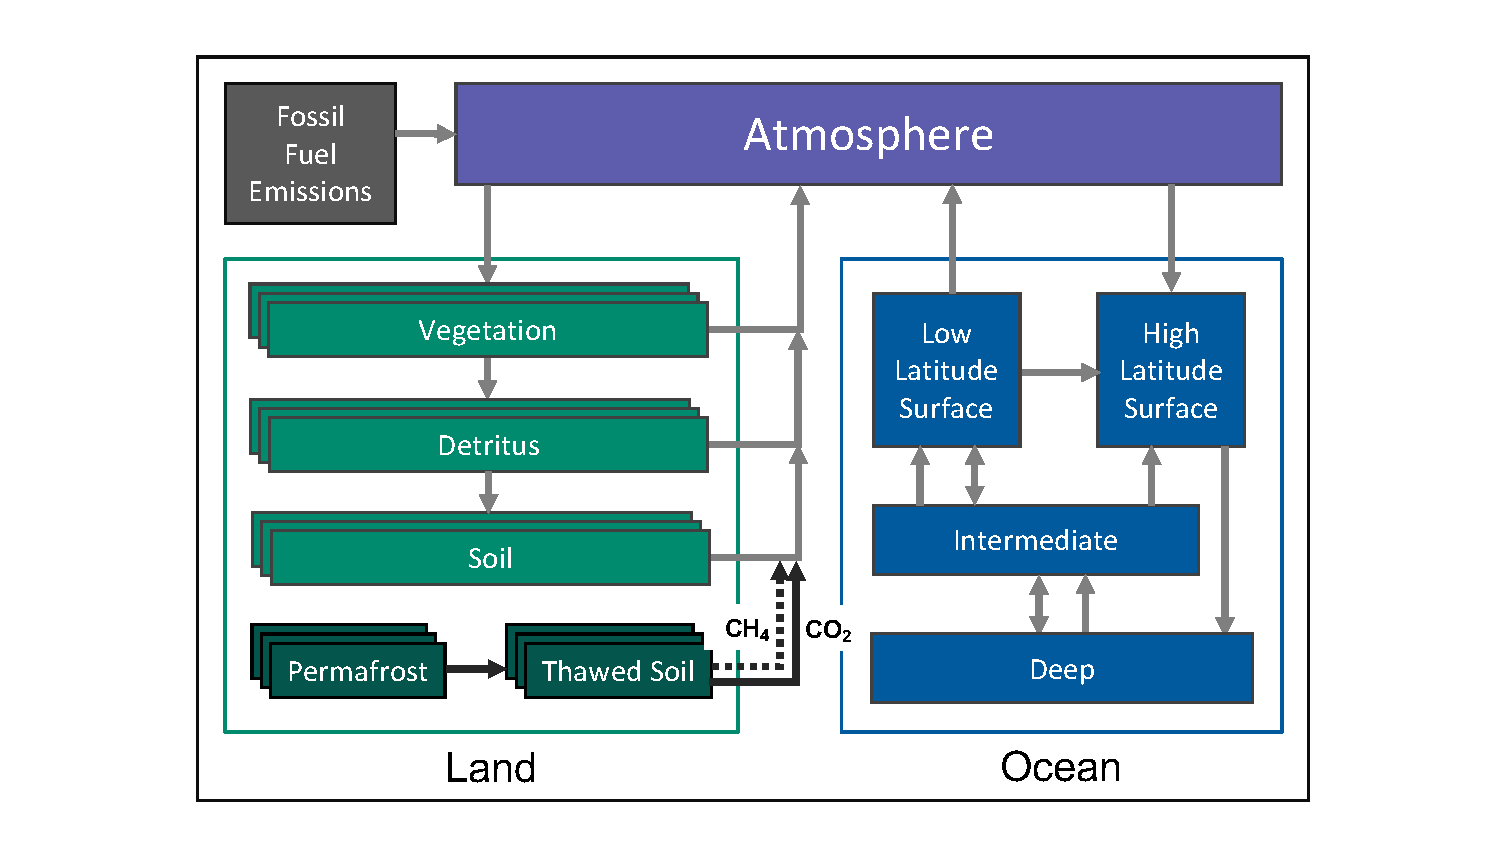
\includegraphics[width=\textwidth]{figures/diagram_perm_ch4_split.pdf}
    \caption{Hector's default carbon cycle showing fluxes (arrows) between each carbon pool. The terrestrial carbon cycle pools can be split into multiple biomes, so these are shown with multiple boxes. In darker green we show the addition of our novel permafrost representation in Hector. As carbon is exchanged in a variety of forms in Hector, the carbon flux arrows do not correspond to any particular carbon compound except where specified beside the emissions from thawed soil.}
    \label{fig:diagram}
\end{figure}

Ocean carbon in Hector is exchanged between the atmosphere and four carbon pools that model both physical circulation and chemical processes in the ocean. Carbon is taken up from the atmosphere in the high latitude surface box which transfers some portion of this carbon to the deep ocean carbon pool. Carbon from there circulates up to the intermediate ocean layer and finally up to the high and low latitude surface pools. Carbon is finally outgased back to the atmosphere from the low latitude surface pool (Figure \ref{fig:diagram}).

Hector's default terrestrial carbon cycle includes three land carbon pools: vegetation, detritus and soil, which can each be divided across multiple user-defined biomes. The vegetation pool takes up carbon from the atmosphere as net primary productivity (NPP), some of which is tranferred into the detritus pool, which can be decomposed and enter the soil carbon pool. All three land carbon pools separately emit carbon back to the atmosphere from land use change, and soil and detritus release additional carbon through decomposition-driven microbial respiration (Figure \ref{fig:diagram}).  

\subsection{Permafrost Submodel}
We have added permafrost in Hector as an additional soil carbon pool that, because it is frozen, does not decompose or otherwise interact with the rest of Hector's carbon cycle until it thaws. At each time step where temperature increases above present day, a warming-driven fraction of permafrost carbon is transferred into a thawed pool, where it is then accessible to microbes for decomposition. 

For a permafrost carbon pool at time $t$, $C_{perm}[t]$, and a thawed permafrost pool, $C_{thawed}[t]$, (both in units of Pg C), permafrost carbon in Hector is exchanged as: 
\begin{align}
&C_{perm}[t] = C_{perm}[t-1] - \Delta C_{perm}[t]\\
&C_{thawed}[t] = C_{thawed}[t-1] + \Delta C_{perm}[t] - F_{thawed-atm}
\end{align}

where $\Delta C_x[t]$ is the change in the carbon pool $x$ at time $t$. Assuming a uniform permafrost carbon density, $\Delta C_{perm}[t]$ is given by:
\begin{equation} 
\Delta C_{perm}[t] = \Delta \Phi[t] C_{perm}[t-1]
\end{equation}

where $\Phi[t]$ is the fraction of permafrost remaining at time $t$ and the change in the frozen fraction at at a particular time step, $\Delta \Phi[t]$, is given by $\Phi[t] - \Phi[t-1]$. To a first approximation, $\Phi[t]$ can be estimated as a function of mean air temperature (global or adjusted by a biome-specific warming factor). Previous work assumes this relationship is linear \citep{kessler_2017_estimating}; 
however, because the permafrost area fraction is, by definition, bounded by zero and one\footnotemark, and because deeper permafrost thaws more slowly than shallow permafrost, we instead use the lognormal cumulative distribution function: \begin{equation}
\Phi[t] = 1 - NCDF(\log(x) | \mu, \sigma)
\end{equation}

where $\mu$ and $\sigma$ are model parameters tuned to most closely fit the linear model used by \citet{kessler_2017_estimating} (Figure \ref{fig:kessler}). 


\footnotetext{Technically, permafrost area could increase in the case of cooling temperatures, and therefore the area fraction could be greater than 1. However, because even the most aggressive climate action scenarios show temperatures that stabilize above year 2000, we assume that permafrost area will never grow more than the starting value.}

\begin{figure}
    \centering
    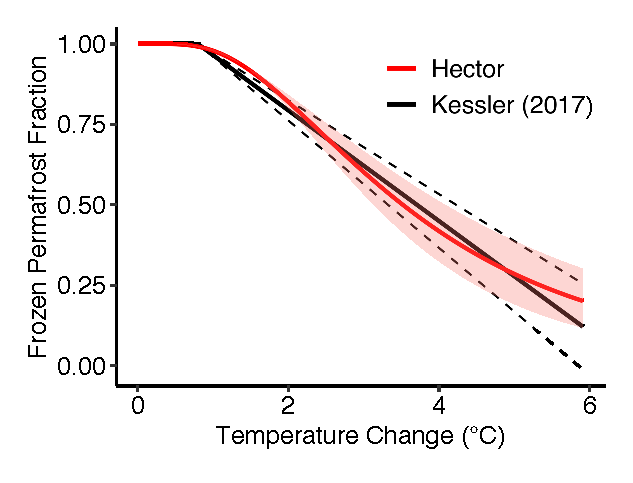
\includegraphics[width=0.8\textwidth]{figures/kessler_calibration.eps}
    \caption{Lognormal permafrost-temperature relationship (red) in Hector compared with linear model used in \citet{kessler_2017_estimating} (black). Dashed lines are the upper and lower bounds of the Kessler model, and the shaded area in red fills the region between lognormal distributions fit to the Kessler upper and lower bounds.}
    \label{fig:kessler}
\end{figure}



\subsubsection{Permafrost Carbon Emissions}
Once thawed, carbon becomes vulnerable to decomposition, generating CO$_2$ and CH$_4$ emissions to the atmosphere from microbial respiration. While carbon in Hector's default soil pool only produces CO$_2$ emissions, we assume a fraction of thawed permafrost is decomposed under anaerobic conditions, consequently releasing a more significant amount of CH$_4$. The partitioning between these two gases is controlled by a respiration fraction, $f_{CH4}$. We also assume that some thawed permafrost carbon is stable and therefore remains invulnerable to decomposition. This non-labile fraction of carbon, $f_{static}$, is removed from the thawed permafrost at each time step before decomposition. 

Total heterotrophic respiration ($RH[i,t]$) for biome $i$ at time $t$ is the sum of heterotrophic respiration in detritus ($RH_d$), soil ($RH_s$), and thawed permafrost ($RH_{pf}$).
\begin{equation} 
RH[i,t] = RH_s[i,t] + RH_d[i,t] + RH_{pf}[i,t]
\end{equation}

Detritus and soil heterotrophic respiration are proportional to the sizes of their respective carbon pools ($C_d$ and $C_s$, respectively, both in Pg C),
with a rate that increases exponentially with temperature according to a biome-specific temperature sensitivity parameter ($Q_{10}$).
Detritus respiration increases with biome-specific air temperature change since pre-industrial ($T[i,t]$),
while soil respiraiton increases with the 200 year running mean of air temperature ($T_{200}[i,t]$) because soils warm slowly relative to the atmosphere. Thawed permafrost respiration behaves identically to soil respiration except for releasing a fraction of the carbon emissions as CH$_4$.
\begin{align}
&T_{air}[i,t] = \delta T_{air}[t] \\
&RH_d[i,t] = \frac{1}{4} C_d Q_{10}[i] ^ {{T}[i,t] / 10} \\
&RH_s[i,t] = \frac{1}{50} C_s Q_{10}[i] ^ {T_{200}[i,t] / 10} \\
&RH_{pf}[i,t] = (1-f_{static})\cdot(1-f_{CH4})\cdot C_{thawed} \cdot Q_{10}[i] ^ {T_{200}[i,t] / 10} \\
&RH_{CH4}[i,t] = (1-f_{static})\cdot(f_{CH4})\cdot C_{thawed} \cdot Q_{10}[i] ^ {T_{200}[i,t] / 10}
\end{align}

In the default configuration of Hector, natural CH$_4$ emissions are prescribed at a constant value (300 Tg year$^{-1}$) \citep{hartin_2015_simple}.
In the new configuration, additional CH$_4$ emissions are added from $RH_{CH4}$.

\subsection{Configuration}
\begin{table}[ht!]
\centering
%\linespread{1.3}
\caption{Hector configuration of permafrost-related parameters and initial values based on literature review.}
 \begin{tabularx}{\textwidth}{l l c c p{1.25in} p{1.75in}} 
 \hline\noalign{\medskip}
Parameter & Hector Nomenclature & Value & Estimated Range & Reference & Description\\ [1ex]
 \hline\noalign{\medskip}
 $\mu$ & \texttt{pf\_mu} & 1.258 & 1.14-1.41 & tuned to \citet{kessler_2017_estimating} & Permafrost-thaw parameter \\ 
 %[1ex]\hline 
$\sigma$ & \texttt{pf\_sigma} & 0.618 & .53-0.71 & tuned to \citet{kessler_2017_estimating} & Permafrost-thaw parameter \\
 %[1ex]\hline 
 $f_{static}$ & \texttt{fpf\_static} & 0.40 & 0.13-0.60 & \citet{burke_2012_uncertainties, burke_2013_estimating} & Non-labile permafrost fraction \\ 
 %\hline
 $C_{perm}(0)$ & \texttt{permafrost\_c0} & 1035 Pg C & 885-1185 Pg C & \citet{hugelius_2014_estimated} & Initial permafrost carbon\\
 %\hline
  $f_{RH\_CH4}$ & \texttt{rh\_ch4\_frac} & 0.023 & 0.01-0.03 & \citet{kessler_2017_estimating} & Fraction of thawed permafrost \mbox{decomposed} as methane \\[1ex] 
 \hline
 \end{tabularx}
 \label{table:config}
\end{table}
Initial permafrost C is set to 1035 ($\pm$ 150) Pg C based on the estimate for near-surface (<3 m depth) permafrost by \citet{hugelius_2014_estimated}. We fit lognormal distribution parameters $\mu$ and $\sigma$ to most closely reproduce the rate of 0.172 ($\pm$ 0.0261) K$^{-1}$ reported by \citet{kessler_2017_estimating} over the range of 0.8 K \footnotemark to 4 K above the pre-industrial baseline. Estimates of the size of the passive pool vary widely but we use a mean of 0.40 (0.13-0.60) based on estimates by \citet{burke_2012_uncertainties, burke_2013_estimating}. The partitioning between methane and carbon dioxide emissions we take to be 2.3\% from \citet{kessler_2017_estimating}.

\footnotetext{\citet{kessler_2017_estimating} report this as temperature change from year 2000. The warming since pre-industrial as estimated by the default Hector configuration is 0.8 K.}

\subsection{Evaluation}
We ran Hector with and without permafrost feedbacks using forcings from each of four Representative Concentration Pathways (RCPs), RCP2.6, RCP4.5, RCP6.0, and RCP8.5 (cite). We chose these scenarios to broadly demonstrate the impacts of a wide range of future climate conditions on permafrost thaw and permafrost-driven carbon emissions. 

Given that much uncertainty remains surrounding permafrost controls, we also ran a sensitivity analysis of the parameters in Table \ref{table:config} over the estimated ranges of each parameter.

\section{Results}

Across the scenarios chosen, the addition of permafrost thaw increases the active soil carbon pool by between XXX and 163 Pg C (in RCP2.6 and RCP8.5, respectively) by 2100, some of which is decomposed and emitted into the atmosphere as CO$_2$ generating a net end-of-century increase of 70 ppm in RCP8.5. resulting in temperature increases above the no-permafrost runs of 0.1-0.2 \degree C across the RCPs. For this figure all the carbon is emitted as CO$_2$, so as Ben said we just want to add a fraction that would be emitted as methane instead.

\begin{figure}
    \centering
    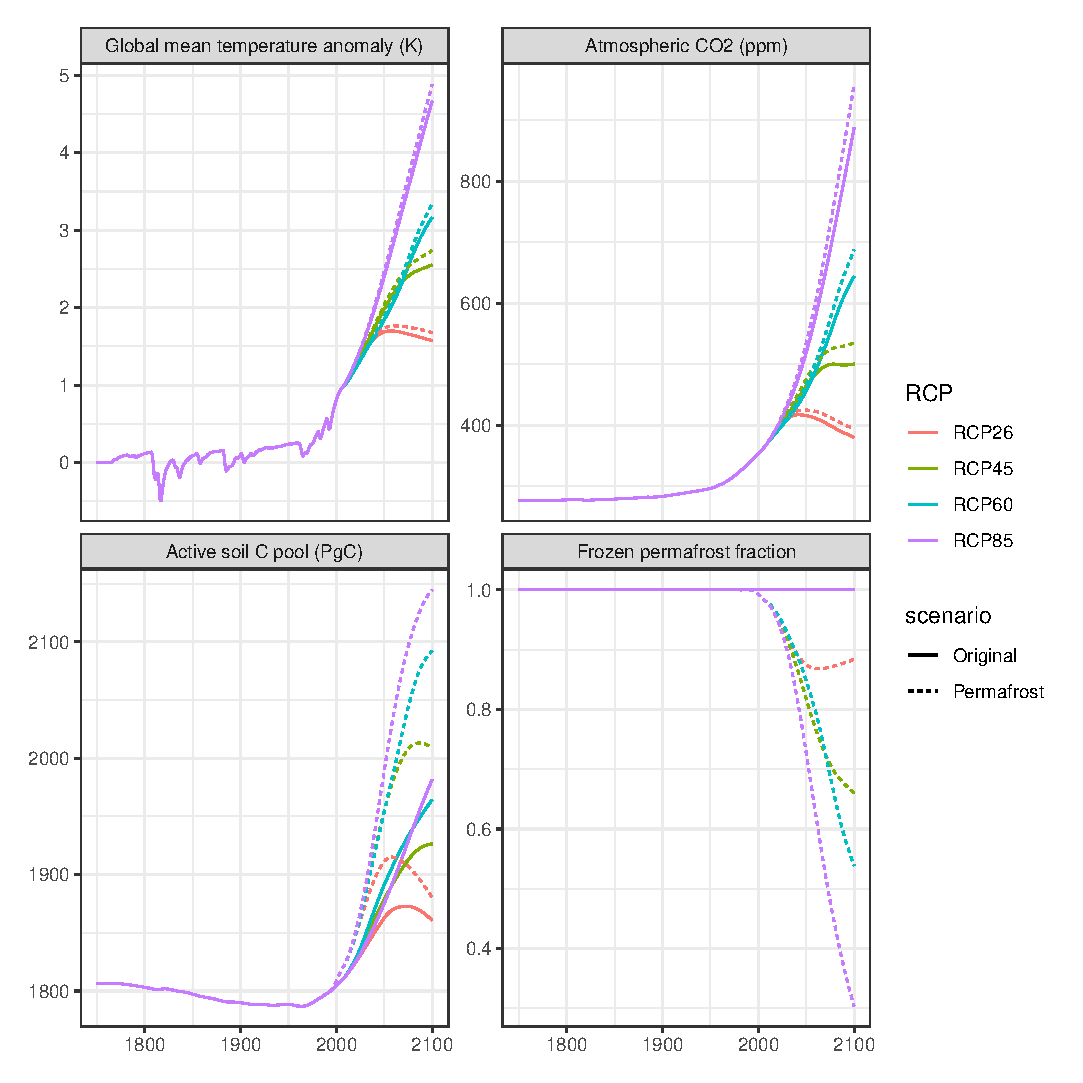
\includegraphics[width=\textwidth]{figures/hector_4panel_results.eps}
    \caption{Carbon and climate effects of the permafrost carbon feedback in Hector.}
    \label{fig:results}
\end{figure}


\subsection{Sensitivity analysis}

The most significant parameter in terms of the net effect 

\begin{figure}
    \centering
    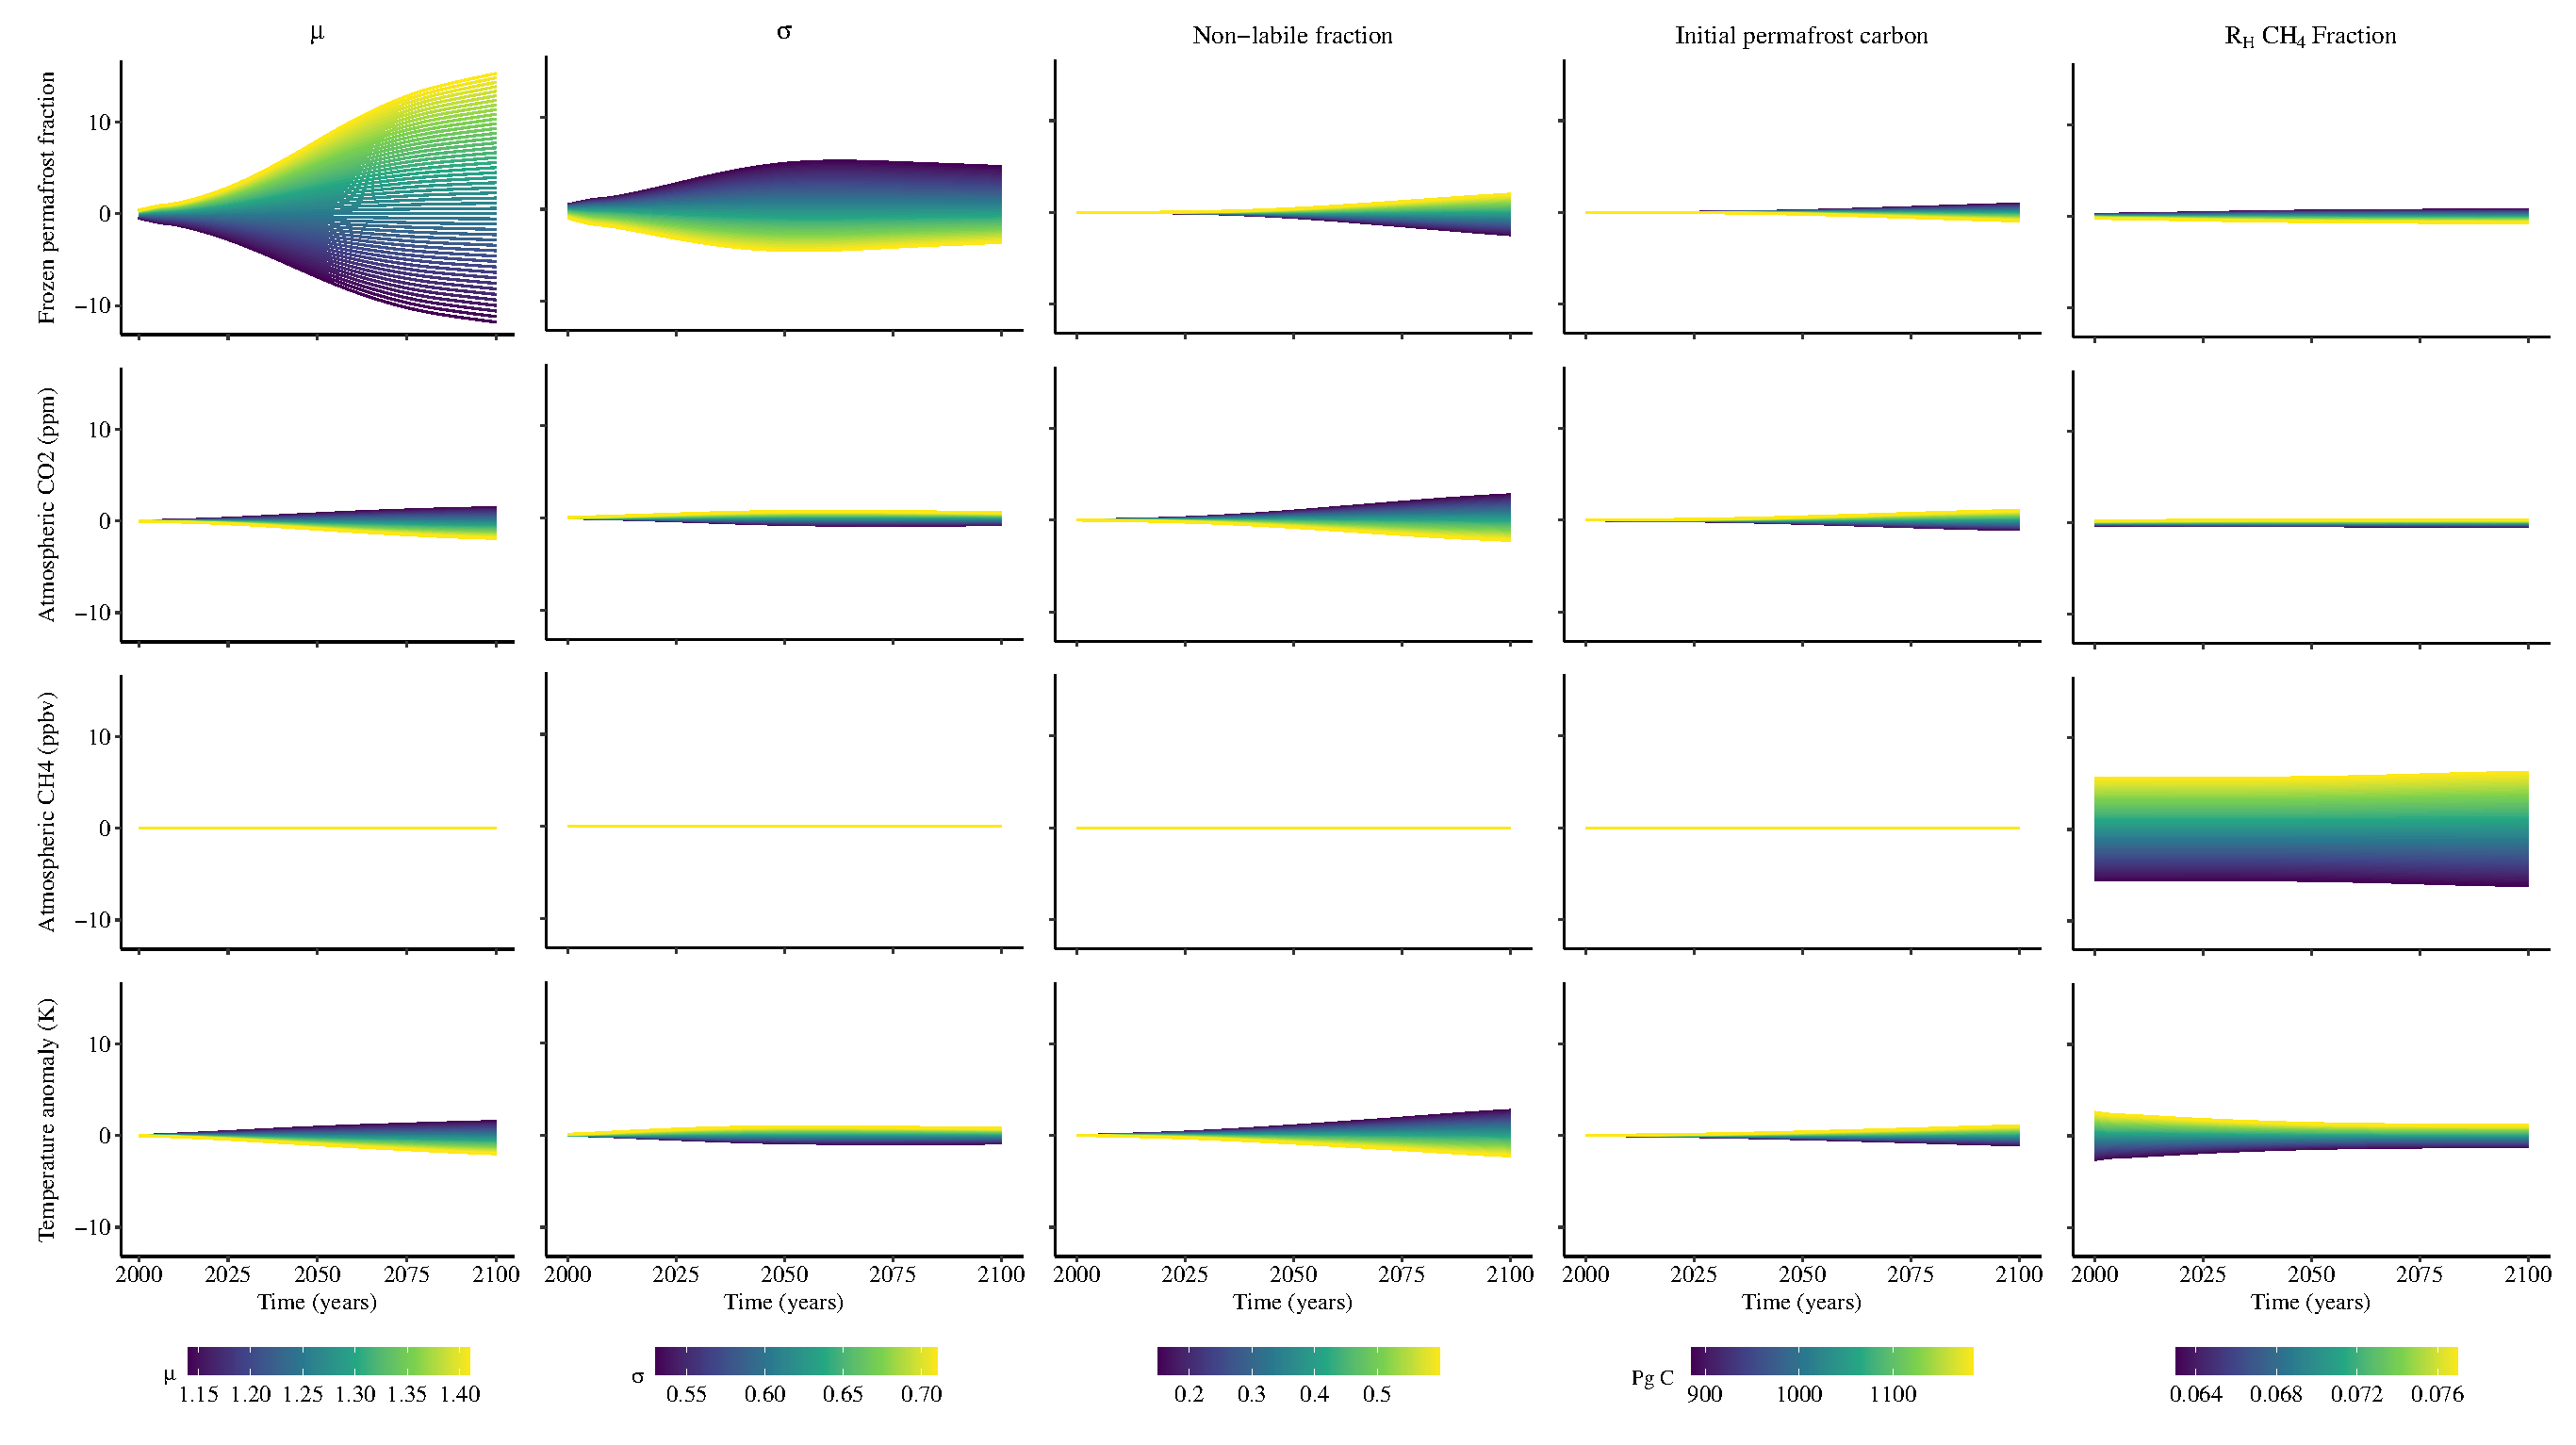
\includegraphics[width=\textwidth]{figures/sensitivity_analysis_all_years.eps}
    \caption{Effect of tuning the permafrost thaw parameters $\mu$ and $\sigma$, the non-labile permafrost fraction, initial permafrost, and the methane fraction of heterotraphic respiration.}
    \label{fig:sensitivity}
\end{figure}


\section{Discussion}
Rate of permafrost C release also depends on soil moisture conditions -- drier soils release C much faster ("carbon bomb") than wetter soils ("carbon fizz") \citep{elberling_2013_long-term}.
Moisture will also affect the balance of aerobic (CO2 release) vs. anaerobic (CH$_4$) C release \citep{turetsky_2002_boreal}, to the extent that unclear if anaerobic (wet) areas are C sources or sinks \citep{wickland_2006_effects}.
Effects of permafrost thaw on soil moisture are a complex hydrological problem -- drainage very sensitive to local (micro-)topography \citep{wickland_2006_effects}.
So will vegetation cover \citep{wickland_2006_effects}.

Temperature amplification of permafrost carbon feedback (by 2100) 0.02 to 0.36 °C \citep{burke_2013_estimating, schneider-von-deimling_2012_estimating, schneider-von-deimling_2015_observation-based}, or 0.1 to 0.8 °C in \citep{macdougall_2012_significant, macdougall_2013_if}, or 10-40\% of peak temperature change \citep{crichton_2016_permafrost}, or 0.2 to 12\% \citep{burke_2017_quantifying}.

Permafrost carbon has greater impact at lower emissions scenarios \citep{burke_2017_quantifying, macdougall_2012_significant, macdougall_2013_if} .


\conclusions  %% \conclusions[modified heading if necessary]
The addition of permafrost thaw in Hector provides an important tool for understanding the potential impact of the permafrost carbon feedback over the next decades and centuries. The model’s simplicity means that it can cheaply run uncertainty analyses over a wide range of parameter values to account for the remaining gaps in our knowledge of permafrost controls. Additionally, Hector's permafrost module can be easily coupled with integrated assessment models like GCAM to estimate the economic consequences of warming from this feedback.



%% The following commands are for the statements about the availability of data sets and/or software code corresponding to the manuscript.
%% It is strongly recommended to make use of these sections in case data sets and/or software code have been part of your research the article is based on.

%\codeavailability{TEXT} %% use this section when having only software code available


%\dataavailability{TEXT} %% use this section when having only data sets available


%\codedataavailability{TEXT} %% use this section when having data sets and software code available


%\sampleavailability{TEXT} %% use this section when having geoscientific samples available


%\videosupplement{TEXT} %% use this section when having video supplements available


%\appendix
%\section{}    %% Appendix A

%\subsection{}     %% Appendix A1, A2, etc.


%\noappendix       %% use this to mark the end of the appendix section

%% Regarding figures and tables in appendices, the following two options are possible depending on your general handling of figures and tables in the manuscript environment:

%% Option 1: If you sorted all figures and tables into the sections of the text, please also sort the appendix figures and appendix tables into the respective appendix sections.
%% They will be correctly named automatically.

%% Option 2: If you put all figures after the reference list, please insert appendix tables and figures after the normal tables and figures.
%% To rename them correctly to A1, A2, etc., please add the following commands in front of them:

%\appendixfigures  %% needs to be added in front of appendix figures

%\appendixtables   %% needs to be added in front of appendix tables

%% Please add \clearpage between each table and/or figure. Further guidelines on figures and tables can be found below.



\authorcontribution{TEXT} %% this section is mandatory

\competinginterests{TEXT} %% this section is mandatory even if you declare that no competing interests are present

%\disclaimer{TEXT} %% optional section

\begin{acknowledgements}
This work was supported by... 
\end{acknowledgements}




%% REFERENCES

\bibliographystyle{copernicus}
\bibliography{references.bib}
%%
%% URLs and DOIs can be entered in your BibTeX file as:
%%
%% URL = {http://www.xyz.org/~jones/idx_g.htm}
%% DOI = {10.5194/xyz}


%% LITERATURE CITATIONS
%%
%% command                        & example result
%% \citet{jones90}|               & Jones et al. (1990)
%% \citep{jones90}|               & (Jones et al., 1990)
%% \citep{jones90,jones93}|       & (Jones et al., 1990, 1993)
%% \citep[p.~32]{jones90}|        & (Jones et al., 1990, p.~32)
%% \citep[e.g.,][]{jones90}|      & (e.g., Jones et al., 1990)
%% \citep[e.g.,][p.~32]{jones90}| & (e.g., Jones et al., 1990, p.~32)
%% \citeauthor{jones90}|          & Jones et al.
%% \citeyear{jones90}|            & 1990



%% FIGURES

%% When figures and tables are placed at the end of the MS (article in one-column style), please add \clearpage
%% between bibliography and first table and/or figure as well as between each table and/or figure.


%% ONE-COLUMN FIGURES

%%f
%\begin{figure}[t]
%\includegraphics[width=8.3cm]{FILE NAME}
%\caption{TEXT}
%\end{figure}
%
%%% TWO-COLUMN FIGURES
%
%%f
%\begin{figure*}[t]
%\includegraphics[width=12cm]{FILE NAME}
%\caption{TEXT}
%\end{figure*}
%
%
%%% TABLES
%%%
%%% The different columns must be seperated with a & command and should
%%% end with \\ to identify the column brake.
%
%%% ONE-COLUMN TABLE
%
%%t
%\begin{table}[t]
%\caption{TEXT}
%\begin{tabular}{column = lcr}
%\tophline
%
%\middlehline
%
%\bottomhline
%\end{tabular}
%\belowtable{} % Table Footnotes
%\end{table}
%
%%% TWO-COLUMN TABLE
%
%%t
%\begin{table*}[t]
%\caption{TEXT}
%\begin{tabular}{column = lcr}
%\tophline
%
%\middlehline
%
%\bottomhline
%\end{tabular}
%\belowtable{} % Table Footnotes
%\end{table*}
%
%%% LANDSCAPE TABLE
%
%%t
%\begin{sidewaystable*}[t]
%\caption{TEXT}
%\begin{tabular}{column = lcr}
%\tophline
%
%\middlehline
%
%\bottomhline
%\end{tabular}
%\belowtable{} % Table Footnotes
%\end{sidewaystable*}
%
%
%%% MATHEMATICAL EXPRESSIONS
%
%%% All papers typeset by Copernicus Publications follow the math typesetting regulations
%%% given by the IUPAC Green Book (IUPAC: Quantities, Units and Symbols in Physical Chemistry,
%%% 2nd Edn., Blackwell Science, available at: http://old.iupac.org/publications/books/gbook/green_book_2ed.pdf, 1993).
%%%
%%% Physical quantities/variables are typeset in italic font (t for time, T for Temperature)
%%% Indices which are not defined are typeset in italic font (x, y, z, a, b, c)
%%% Items/objects which are defined are typeset in roman font (Car A, Car B)
%%% Descriptions/specifications which are defined by itself are typeset in roman font (abs, rel, ref, tot, net, ice)
%%% Abbreviations from 2 letters are typeset in roman font (RH, LAI)
%%% Vectors are identified in bold italic font using \vec{x}
%%% Matrices are identified in bold roman font
%%% Multiplication signs are typeset using the LaTeX commands \times (for vector products, grids, and exponential notations) or \cdot
%%% The character * should not be applied as mutliplication sign
%
%
%%% EQUATIONS
%
%%% Single-row equation
%
%\begin{equation}
%
%\end{equation}
%
%%% Multiline equation
%
%\begin{align}
%& 3 + 5 = 8\\
%& 3 + 5 = 8\\
%& 3 + 5 = 8
%\end{align}
%
%
%%% MATRICES
%
%\begin{matrix}
%x & y & z\\
%x & y & z\\
%x & y & z\\
%\end{matrix}
%
%
%%% ALGORITHM
%
%\begin{algorithm}
%\caption{...}
%\label{a1}
%\begin{algorithmic}
%...
%\end{algorithmic}
%\end{algorithm}
%
%
%%% CHEMICAL FORMULAS AND REACTIONS
%
%%% For formulas embedded in the text, please use \chem{}
%
%%% The reaction environment creates labels including the letter R, i.e. (R1), (R2), etc.
%
%\begin{reaction}
%%% \rightarrow should be used for normal (one-way) chemical reactions
%%% \rightleftharpoons should be used for equilibria
%%% \leftrightarrow should be used for resonance structures
%\end{reaction}
%
%
%%% PHYSICAL UNITS
%%%
%%% Please use \unit{} and apply the exponential notation


\end{document}
